\section{Results}

\subsection{Single-shot model performance}
\label{subsection:single-shot}
% How did we come up with linear models:
% 	- compare performance of all models by "recall"
% 	- compare time with the actual docking time
% 	- test effects of normalization

In order to select most promising models for active-learning iterations, we first compared them on a single batch (figure \ref{fig:fig_4}). 

First, we selected diverse regression models (figure \ref{fig:fig_4}, first row), and compared them with lower-bond and upper-bond baselines. Namely, we trained the regression models to predict the docking score directly, then selected top-1\% from the sorted list as model's hits, and compared model's hits with actual top-1\% of the list. Lower-bond baselines included sklearn's DummyRegressor, as well as custom models yielding random score from either normal or uniform distribution, matching original distribution of scores (RandomUniform and RandomGaussian regressors, respectively). For upper-bond baseline, we used docking scores, provided by the second run of Molsoft's ICM (figure \ref{fig:fig_1}) without fixing a seed value.

From this run, it is clear that linear regression performs at the level of more sophisticated models. Thus, we selected these models to test on dataset of 5zty docking scores. Surprisingly, linear regression itself showed baseline performance, while it's weighted versions, such as Lasso and Ridge regression, performed at the level with more sophisticated models.

Last, we tested both sophisticated regression models and linear models, on known datasets obtained with DOCK \cite{ultralarge_docking_first}. As expected, different models show comparable recall, that also becomes more reproducible with the increase of the train size dataset. More complex models such as RandomForestRegressor show superior performance compared to more simple models. 

Single-batch models share multiple trends for all models and train sizes. First, all models outperform the random baselines, as expected. Surprisingly, linear models with and without regularization don't differ by their performance. For more complicated models such as random forest and decision tree regressors, an increase in prediction quality with increase of model training size. 

Paragraph about effect of normalization

\begin{figure}[h]
% Fig 4: selection of the best single model
% 	- A: model performances
% 	- B: model timing
% 	- C: time vs performance distribution + actual docking time cutoff
\centering
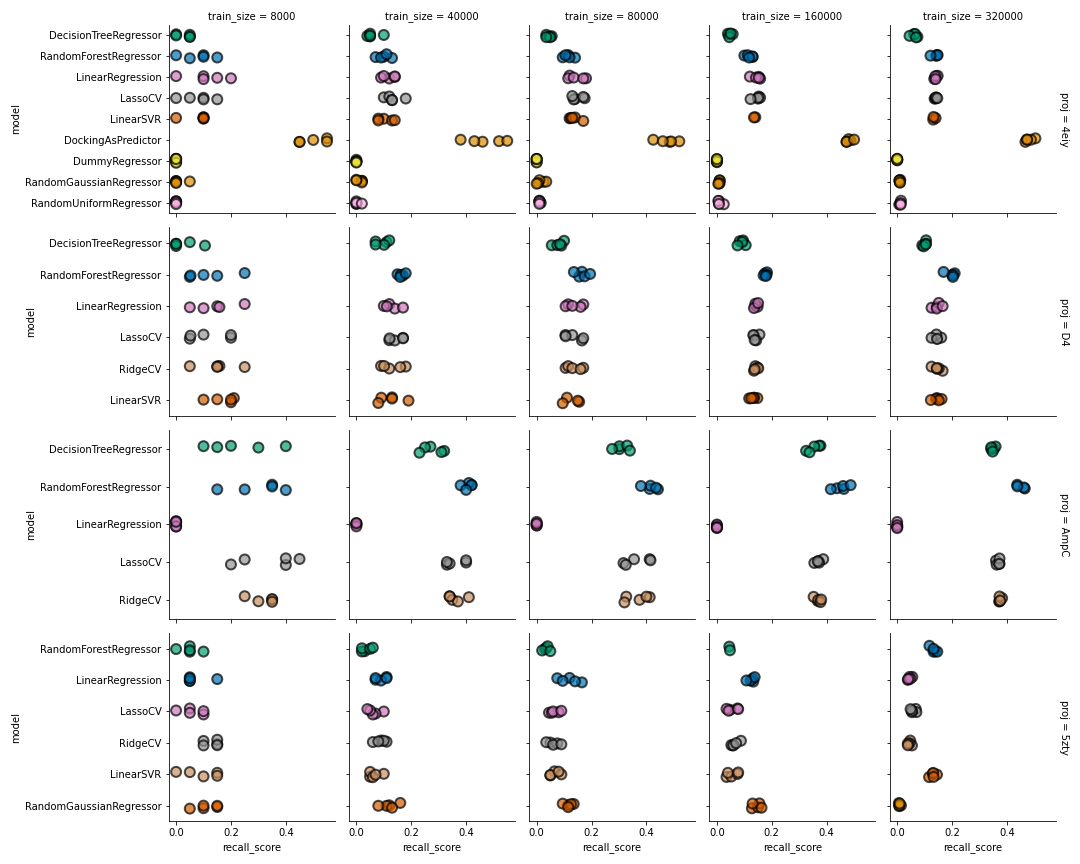
\includegraphics[width=0.8\textwidth]{figures/Figure_4.png}
\caption{Model performance for multiple regression models and their baselines on 4 datasets present in the study. \texttt{recall\_score} shows the share of interception of top-1\% of the regressor's predictions with the actual top-1\%, sorted by docking score}
\label{fig:fig_4}
\end{figure}

\subsection{Optimization of active learning regime}

To optimize meta-parameters of the active learning regime, we selected LinearRegression as the "base" learner. The choice was based on it's superior speed (see fig. TODO) and performance comparable with more complex models (figure \ref{fig:fig_3}). Active learning models were compared by their ability to retrieve top-1\% hits from the \texttt{4eiy} dataset, and compared with upper-and lower-bond baselines, as described in \ref{subsection:single-shot}. Each model had a fixed batch per single iteration, so that exactly \texttt{train\_size} scores were added to the training data on each iteration. Also, we tested the effect of the increasing (\texttt{add\_to\_train=True}) or constant (\texttt{add\_to\_train=False}) training dataset size, with the latter presumably providing the ability for the model to escape local minima in the chemical space. Finally, we tested the selection regime for the next batch: with \texttt{LastModel}, only the model from the previous batch was taken into account; with \texttt{MeanRank}, the mean molecule rank among models on all iterations was used as its score; and with \texttt{TopFromEveryModel}, all models from all iterations contributed equal amount of molecules to the next batch.


% How did we come up with iterations scheme:
% 	- compared different train sizes
% 	- compared different regimes (add/noadd)
% 	- compared different ensembling methods
% 	- compare with "docking-as-predictor"

\begin{figure}[h]
% Fig 5: fine-tuning metaparameters of "iterations" 
% 	- batch size effect on the iterations performance
% 	- add/noadd & different ranking schemes effect
% 	- comparison  of the best model with with docking-as-predictor
% 	- TODO: comparison with the really best single model
\centering
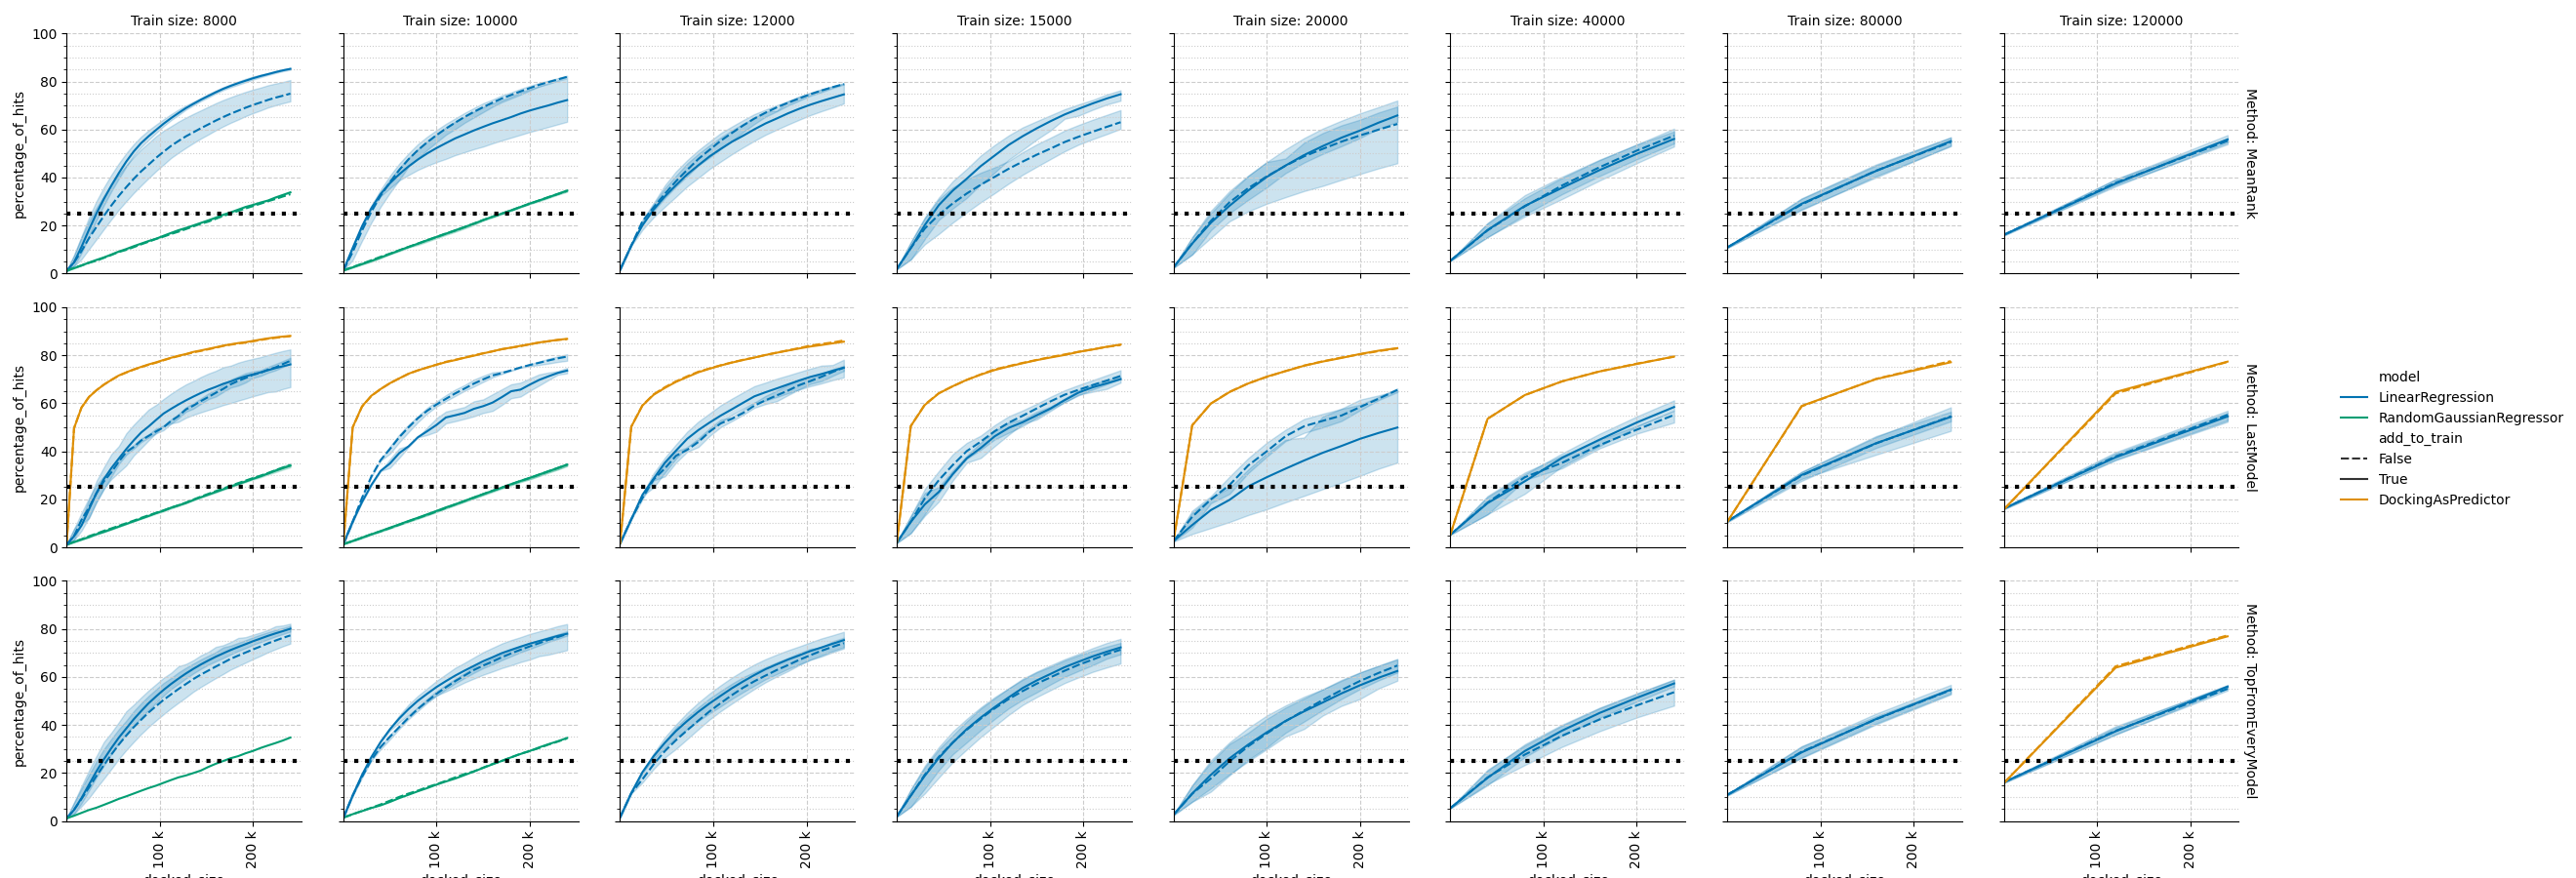
\includegraphics[width=0.8\textwidth]{figures/Figure_3_4eiy.png}
\caption{Model performance in active learning regime}
\label{fig:fig_3}
\end{figure}

Interestingly, the \texttt{train\_size} effect for the active learning regime was different from the single-batch mode. Namely, smaller training size resulted in better model performance regardless of other active learning meta parameters (figure \ref{fig:fig_3}). Smallest training size of $8~000$ resulted in retrieval of $\approx80\%$ of top-1\% molecules, while largest training size of $120~000$ resulted in mere $\approx60\%$, even though mean recall for a single-batch regime is $0.11(7)$ and $0.15(1)$, respectively. Besides, neither the next batch selection regime nor the \texttt{add\_to\_train} parameter do not have an influence within the observed data.

Paragraph about comparison with upper- and lower-bonds.

Paragraph about comparison of upper-bond between selection regime (probably one selection  regime is just better than the other one, if we have "ideal" data).